\TOWRITE{SL}{Proofread 3.3 pass 1}
\TOWRITE{ALL}{Proofread 3.3 pass 2}
\label{sect:mgt}

\subsubsection{Management}

The project will be coordinated by the University Paris-Sud (UPSud),
represented by Prof. Nicolas Thiery (Project Coordinator), who has
experience in successfully managing several research projects on the
main \TheProject topics.  Pioneer in community-developed open source
software for research in this field, Thiery founded in 2000 the
Sage-Combinat software project involving 50 researchers in Europe and
abroad.  This project has grown under his leadership to be one of the
largest organized communities of Sage developers.

The Project Coordinator will be assisted by a part-time (50\%) Project
Manager, that will be hired for this project and located in the
European Affairs and Technology Transfer Office (SAIC) of the UPSud.
Additional feedback and expertise will be brought by Financial, Legal
and European affairs officers from SAIC.

\subsubsection{Organizational structure and decision-making}

\TOWRITE{Eugenia}{Add organisational structure figure}

The organizational structure, shown in the Figure XXXXXXX, has been designed
to enable efficient coordination of the \TheProject project --- a VRE
integrating several previously separated tools and software and
involving both academic actors and industrial stakeholders.

We have designed the management structure and procedures to deal in a
flexible manner with the following challenges:

\begin{itemize}
\item to integrate all consortium members and to mobilize their
  expertise, knowledge and networks at every stage of the project;
\item to give the maximum attention to the end-users needs and
  requirements;
\item to continuously involve expertise and knowledge of relevant
  stakeholders and their networks, and
\item to efficiently coordinate the project implementation in a
  collaborative environment and ensure its sustainability.
\end{itemize}

The coordinator is acting as an intermediary between the Partners and
the European Commission. The coordinator will oversee the project
planning, monitor that the execution is carried out in time and that
the objectives are achieved and closely interact with the project
officer for the project monitoring and delivering the performance
indicators.  The Project Manager will ensure an efficient day-to-day
management of the project, reporting, feedback to partners on
administrative, financial and legal issues, follow-up of the resources
allocation and consumption, communication inside and outside the
consortium.

The resources of all partners will be mobilized by decentralisation of
responsibilities through the assignment of leadership for work
packages. A clear task sharing obtains efficient decision making
mechanisms and a sound financial management will safeguard the
achievement of the project’s objectives.

\subsubsection{Project roles}

The following bodies will form the organizational structure of the
\TheProject project : Coordination Team (MT), Steering Committee (SC),
Advisory Board (AB), End User Group (EUG) and Quality Review board
(QRB).


\paragraph{Coordination Team (CT)} 
\subparagraph{Members:} The CT is composed of the Work Package leaders
and headed by the Project Coordinator, assisted by the Project
Manager.

\subparagraph{Responsibilities:} CT is an executive body in charge of
the project implementation and monitoring.

It takes operational decisions necessary for the smooth execution of
the project.

Tasks:
\begin{compactenum} 
\item Monitoring the timely execution of the tasks and achievement of
  the objectives;
\item Preparing of scientific and financial progress reports;
\item Controlling the WP progress by assessing it through technical
  reports developed by the WP partners;
\item Making proposals to the Steering Committee of re-allocation of
  tasks, resources and financial needs for the fulfilment of the work
  plan;
\item Preparing the drafts and validating the project deliverables to
  be submitted to the Commission; Meetings : Project Coordinator and
  Project Manager can meet any time and at least twice a week. They
  will meet Work-Package leaders every 6 months. If necessary,
  extra-meetings will be arranged.
\end{compactenum} 

\paragraph{Steering Committee (SC)}

\subparagraph{Members:} The SC is chaired by the Project Coordinator
and includes one representative from each partner organization.

\subparagraph{Responsibilities:} The SC is the decision-making body in
charge of its strategic orientation.  It takes decisions on scientific
orientations of the project, re-allocation of resources, consortium
changes, intellectual property rights

\subparagraph{Meetings:} Every 6 months. If necessary, extra-meetings
will be arranged.  Written minutes of each meeting will be produced,
which shall be the formal record of all decisions taken. A procedure
for comment and acceptance is proposed.

\subparagraph{Voting procedure:} The SC shall not deliberate until all
Members are present or represented.  Each Member shall have one
vote. The GA will work on consensual decisions as much as possible and
resort to voting only if unavoidable. Voting decisions shall be taken
by a majority of two-thirds (2/3) of votes.

\paragraph{Advisory board (AB):}

\subparagraph{Members:} top level experts from partner organizations
and external, including both experts from the project scientific area,
and experts on legal and social matters.

\subparagraph{Responsibilities:} to give an independent opinion on
scientific and innovation matters, in order to guaranty quality
implementation of the project, efficient innovation management and
project sustainability.  Meetings : on the demand of the Steering
Committee.

\paragraph{Quality Review Board (QRB)}
\subparagraph{Members:} The QRB will be composed of 2 senior
researchers from the Consortium, 2 representatives of the End User
Group and 2 experts from the Advisory Board. It will be chaired by one
of the professors within the Consortium. All members will be appointed
at kick-off meeting of the project.  
\subparagraph{Responsibilities:}
to monitor the quality of the Deliverables, the whole ‘production
process’ and to recommend improvements during the project to the SC.
\subparagraph{Meetings:} before publications and reports of the
project.

\paragraph{End User Group (EUG)}
\subparagraph{Members:} end-users of the VRE, internal and external to
the consortium, from different disciplines and both from academic and
industrial sector. They are actively involved into the project
execution, and work in close interaction with the project coordinator.

\subparagraph{Responsibilities:} the EUG is the main actor of the innovation
management within the consortium, as they have a deep understanding of
both market and technical problems, and awareness of
opportunities. The EUG also plays a main role in ensuring the VRE
sustainability.  

\subparagraph{Tasks:} to control the project execution from the
point of view of the end user needs and requirements, to test the tool
and to detect its potential shortcomings at the early stages, to
propose adaptation measures.  Meetings : the EUG will have regular
virtual meetings, and will meet physically at least once a year.


\subsubsection{Project management tools and procedures}

Project partners and management bodies will communicate through
especially dedicated project web platform, maintained by the Project
Manager. WP leaders will at least monthly monitor progress of
participants of their WP, and participants will inform their WP
leaders when problems are encountered. Major problems will be
discussed in (teleconference) meetings with the project Coordinator
and Project Manager. Each WP leader will be free to organize
extra-meetings with WP partners, if necessary. Scientific and
financial progress reports will be collected, assembled and
transmitted to the Project coordinator by the WP leaders through the
web platform. On basis of the Progress Reports, the Coordination Team
will monitor progress of the project, identify bottlenecks and find
solutions for these problems. Where needed, adaptations to the project
plan will be made, with the aim to ensure the delivery of the project
results as agreed with the EC. Major adaptations need to be approved
by the Steering Committee.  If necessary, the SC can submit reports to
the QRB for opinion.

Finally, the End Users Group, working in close cooperation with the
project coordinator, will ensure the efficient innovation
management. They will carefully monitor the new opportunities, in
order to give, if necessary, new orientations to the project. For
legal aspects, they will have a feedback from legal officers from the
Coordinator’s European Affairs and Technology Transfer office (SAIC),
specialized in Intellectual Property.



Our management structure and procedures will ensure that our network
of 16 partners from both academic and industrial sectors is focused at
achieving the promised deliverables, efficiently managing the
innovation process and largely opening the VRE to its final users. The
15 EU-partners will sign a Consortium Agreement, in which operational
rules and decision making procedures will be laid down. The
international partner will work with a bi-lateral agreement with the
Coordinator.







\subsubsection{Risk management}\label{sec:risks}

The risk in the project execution as planned is carefully assessed and
managed. We base our plans on long standing experience, and we bring
together the world's experts in the relevant tools and techniques.

A key feature of this project is the involvement of a wide set of
partners from multiple domains. While this ensures complementary
coverage of a wide set of skills and provides robustness in different
ways, we will have to ensure that all partners work as closely knit
team. 

Our open source approach means that all our code and outputs
are open and visible to anybody at sites like github and bitbucket
throughout the project. In particular, it is common for users of
computational software to use the most leading edge versions, thus
beta-testing code in-between major releases. This results in risk
reduction: where our design decision or technical approaches are
controversial, this will be detected early by those users, giving the
consortium useful feedback to consider.

The project coordinator will, with support from the Coordination Team
and Quality Review Board, create a Risk Management Plan
\delivref{management}{ipr} as part of the Management Work Package,
which will be reviewed annually.

\noindent
\begin{center}
\begin{tabular}{|m{.3\textwidth}|m{.2\textwidth}|m{.4\textwidth}|}\hline
  Risk & Level with/without mitigation & Mitigation measures\\\hline

  Recruitment of highly qualified staff & High/Medium &
  Great care was taken identifying pool of candidates to hire from,
  and coordinating with currently running projects to rehire personnel
  with strong track record. Typically, we will rehire European
  postdocs that are currently funded by the Sloan grant to work on
  Jupyter in California and wish to come back to Europe.\\\hline

  \TOWRITE{NT}{Not sure about this line (HF) -- remove?} 

  Harming the future
  academic career of young researchers by overwhelming them with technical work & High/Low &
  Great care will be taken in distinguishing PhD and postdocs that
  wish to pursue an academic carrier and full time developers, and
  assigning to the former tasks with a strong research aspect that
  will lead to publications (typically in computer science).\\\hline

  Different groups not forming effective team & Medium/Low & Long track record of working collaboratively on code across multiple sites; Aggressive planning of project meetings, work-shops and one-to-one partner visits to facilitate most effective teamwork, combining face-to-face time at one site with remote collaboration.\\\hline % this also justifies our generous travel budget.

  Implementing infrastructure that does not match the needs of end users & High/Low &
  Most of the members of the consortium are themselves end-users with
  a diverse range of needs and points of views; hence the design of
  the proposal and the governance of the project is naturally steered
  by demand; besides, because we provide a toolkit, users have the
  flexibility to adapt the infrastructure to their needs.\\\hline

  Lack of predictability for tasks that are pursued jointly with
  the community & Medium/Low &
  The PI's have a strong experience managing community-developed
  projects where the execution of tasks depends on the availability of
  partners. Some tasks may end up requiring more manpower from
  \TheProject to be completed on time, while others may be entirely
  taken care of by the community. Reallocating tasks and redefining
  work plans is common practice; this anyway happens to cater for a
  fast evolving context. Such random factors will be averaged out over
  the large number of independent tasks.
\end{tabular}
\end{center}
\TOWRITE{NT/Eugenia}{Impredictability}

%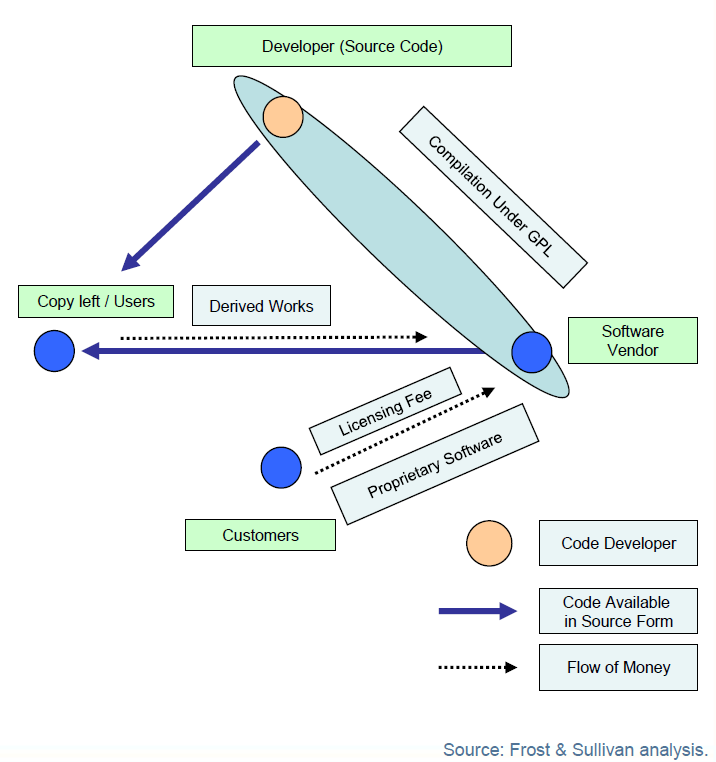
\includegraphics[width=.94\textwidth]{Pictures/Impact-img1.png}

%   But: since Open Source softwares are freely accessible, security
%   and privacy issues are a concern. Anytime a resource is shared,
%   there is greater risk of unauthorised access and contaminated data.
%   Providers must demonstrate security solutions, which should include
%   physical security controlling access to the facility and protection
%   of user data from corruption and cyber attacks.}


%  LocalWords:  mgt Paris-Sud UPSud Thiery Sage-Combinat decentralisation textwidth hline
%  LocalWords:  textwidth Jupyter slmhnlnhfnhs hsfhs ghshsh includegraphics unauthorised

%%% Local Variables:
%%% mode: latex
%%% TeX-master: "proposal"
%%% End:
